\documentclass[a4paper, 11pt]{article}
\usepackage{graphicx} % Required for inserting images
\usepackage{amsmath}
\usepackage{geometry}
\usepackage{hyperref}
\usepackage{setspace}
\usepackage{array}
\usepackage[usenames,dvipsnames]{xcolor}
\usepackage{colortbl} 
\usepackage{tabularray}
\usepackage[italian]{babel}

 \geometry{
 a4paper,
 left=25mm,
 right=25mm,
 top=20mm,
 bottom=20mm,
 }

\setlength{\parskip}{1em}
\setlength{\parindent}{0pt}
\graphicspath{{../media/}}

\begin{document}

\begin{minipage}{0.35\linewidth}
    \includegraphics[width=\linewidth]{Logo_Università_Padova.svg.png}
\end{minipage}\hfil
\begin{minipage}{0.55\linewidth}
\textbf{Università degli Studi di Padova} \\
Laurea in Informatica \\
Corso di Ingegneria del Software \\
Anno Accademico 2023/2024
\end{minipage}

\vspace{5mm}

\begin{minipage}{0.35\linewidth}
    
\includegraphics[width=\linewidth]{logo rotondo.jpg}
\end{minipage}\hfil
\begin{minipage}{0.55\linewidth}
\textbf{Gruppo:} SWEet16 \\
\textbf{Email:} 
\href{mailto:sweet16.unipd@gmail.com}{\nolinkurl{sweet16.unipd@gmail.com}}
\end{minipage}

\vspace{15mm}

\begin{center}
\begin{Huge}
        \textbf{Piano di Qualifica} \\
        \vspace{4mm}
        
\end{Huge}

\vspace{20mm}

\begin{large}
\begin{spacing}{1.4}
\begin{tabular}{c c c}
   Redattori:  &  Alex S. & \\
   Verificatori: & Alberto M. &  \\
   Amministratore: & Alex S. & \\
   Destinatari: & T. Vardanega & R. Cardin \\  
   Versione: & 0.1.0 & 
\end{tabular}
\end{spacing}
\end{large}
\end{center}

\pagebreak

\begin{huge}
    \textbf{Registro delle modifiche}
\end{huge}
\vspace{5pt}

\begin{tblr}{
colspec={|X[1.5cm]|X[2cm]|X[2.5cm]|X[2.5cm]|X[5cm]|},
row{odd}={bg=white},
row{even}={bg=lightgray},
row{1}={bg=black,fg=white}
}
    Versione & Data & Autore & Verificatore & Descrizione \\
    0.1.0 & 2024/02/14 & Alex S. & Alberto M. & Approvazione per rilascio \\
    \hline
  
\end{tblr}

\pagebreak
\tableofcontents
\pagebreak 

\section{Introduzione e scopo del documento}

    \subsection{Scopo del documento}

    Il presente documento si pone lo scopo di individuare e definire le \emph{best practices}$^{G}$ e il \emph{Way of Working}$^{G}$ del progetto che ogni componente del gruppo SWEet16
    si impegna a rispettare durante l’intero svolgimento del progetto Easy Meal. \\
    In questo modo si cercherà di garantire omogeneità e coesione in ogni aspetto del suddetto progetto.
  
    \subsection{Scopo del prodotto}

    Lo scopo dell’applicazione è quello di creare una piattaforma che permetta di gestire e semplificare il processo di \emph{prenotazione}$^{G}$ di tavoli all’interno dei ristoranti. \\
    Sarà inoltre possibile anticipare l’esperienza culinaria visionando prima il menù ed andando ad effettuare la propria \emph{ordinazione}$^{G}$ prima di arrivare al ristorante. \\
    Il prodotto offre inoltre un’esperienza di ordinazione delle \emph{pietanze}$^{G}$ collaborativa e coinvolgente, permettendo di condividerla con amici ed, in caso di dubbi, interagire direttamente con lo staff del ristorante.

    L’idea è una piattaforma \emph{SaaS (Software as a Service)}$^{G}$, in cui i saranno presenti due tipi di utenti:
    \begin{itemize}
      \item \emph{Clienti}$^{G}$: utente registrato all’interno dell’applicazione, può cercare ristoranti, effettuare prenotazioni, ordinazioni e inserire feedback e recensioni;
      \item \emph{Ristoratori}$^{G}$: utente registrato all’interno dell’applicazione, può gestire uno o più ristoranti, controllando le prenotazioni e le ordinazioni dei clienti ed i menù del/i ristorante/i.
    \end{itemize}


    La piattaforma dovrà essere  disponibile attraverso una \emph{WebApp}$^{G}$ accessibile da qualsiasi dispositivo, esso sia \emph{Desktop}$^{G}$ o \emph{Mobile}$^{G}$.
    

    \subsection{Glossario}

    Al fine di evitare possibili ambiguità o incomprensioni riguardanti la terminologia usata nel documento, è stato deciso di adottare un glossario in cui vengono riportate le varie definizioni.  \\
    In questa maniera in esso verranno posti tutti i termini specifici del dominio d’uso con relativi significati. \\
    La presenza di un termine all’interno del glossario viene indicata applicando una " $^{G}$ " ad apice della parola.


    \subsection{Maturità del documento}

    Il presente documento è redatto con un approccio incrementale al fine di poter trattare nuove o ricorrenti questioni in modo rapido ed efficiente, sulla base di decisioni concordate tra tutti i membri del gruppo.  \\
    Non può pertanto essere considerato definitivo nella sua attuale versione.

    \subsection{Riferimenti}

        \subsubsection{Riferimenti normativi}

        \begin{itemize}
            \item Regolamento del progetto didattico: \\
            \url{https://www.math.unipd.it/~tullio/IS-1/2023/Dispense/PD2.pdf}
          \item \emph{Capitolato d’appalto}$^{G}$ C3 - Easy Meal: \\
            \url{https://www.math.unipd.it/~tullio/IS-1/2023/Progetto/C3.pdf}
        \end{itemize}
        
        \subsubsection{Riferimenti informativi}

        \begin{itemize}
            \item I processi di ciclo di vita del software: \\
            \url{https://www.math.unipd.it/~tullio/IS-1/2023/Dispense/T2.pdf}
            \item Glossario: \\
            \url{} %aggiungere link a glossario
        \end{itemize}

        Tutti i riferimenti (normativi e informativi) a risorse web soggette a variazione sono stati consultati il 2024/02/19.


\section{Qualità di processo}
\subsection{Scopo}
La qualità di un prodotto è influenzata dalla qualità dei processi che lo compongono. \\
È quindi necessario dotarsi di metriche che permettano di valutare tali processi e garantire che essi
raggiungano gli obiettivi di qualità fissati.\\
Per garantire una corretta implementazione ed un mantenimento costante, si seguirà
il \textit{ciclo di Deming}, meglio conosciuto come PDCA, che prevede un approccio iterativo funzionale
all'attuazione di un miglioramento continuo.\\
In questa sezione si espongono le metriche scelte ed i livelli di qualità accettabili e ottimali per ciascuna
di esse.\\
Le metriche hanno un identificativo avente come prefisso l'acronimo QPC (Qualità Processo) seguito dal codice della singola metrica.\\

\subsection{Processi primari}

\subsubsection{Fornitura}
\subsubsubsection{Metriche}
\begin{itemize}
    \item \textbf{Budget at Completion (QPC-BAC)}: Totale preventivato del progetto.
\end{itemize}

\begin{itemize}
    \item \textbf{QPC-AC - Actual Cost}: Costo sostenuto per il progetto al momento del calcolo;
    \item \textbf{QPC-ETC - Estimated to Completion}: Stima del valore per la realizzazione delle rimanenti attività;
    \item \textbf{QPC-EAC - Estimated at Completion}: Costo finale stimato alla data della misurazione, revisione del \textbf{QPC-BAC}; $$Formula: \textrm{QPC-AC} + \textrm{QPC-ETC}$$
    \item \textbf{QPC-EV - Earned Value}: Importo guadagnato per il lavoro svolto al momento del calcolo; $$Formula: (\%Lavoro \enspace svolto) \cdot QPC-EAC$$
    \item \textbf{QPC-PV - Planned Value}: Importo pianificato in base al lavoro svolto, al momento del calcolo; $$Formula: (\%Lavoro \enspace pianificato) \cdot \textrm{QPC-BAC}$$
    \item \textbf{QPC-SV - Schedule Variance}: Stato (anticipo/ritardo) della pianificazione. Un valore negativo indica che si è in ritardo rispetto alla pianificazione; $$Formula \enspace base: \textrm{QPC-EV} - \textrm{QPC-PV}$$ $$Formula \enspace in \enspace \%: \textrm{QPC-EV} / \textrm{QPC-PV} \cdot 100$$
    \item \textbf{QPC-CV - Cost Variance}: Differenza tra il budget a disposizione e quello effettivamente utilizzato. Un valore negativo indica che si sta lavorando in perdita. $$Formula: \textrm{QPC-EV} - \textrm{QPC-AC}$$ $$Formula \enspace in \enspace \%: \textrm{QPC-EV} / \textrm{QPC-AC} \cdot 100$$
\end{itemize}
\subsubsubsection{Obiettivi}
\begin{table}[H]
    \begin{tblr}{
        colspec={|X[3cm]|X[5cm]|X[4cm]|X[3cm]|},
        row{odd}={bg=white},
        row{even}={bg=lightgray},
        row{1}={bg=black, fg=white}
}
        Metrica & Descrizione & Valore accettabile & Valore ideale \\
        QPC-AC & Actual Cost & & \\
        QPC-ETC & Estimated to Completion & ${\geq}$ 0\% & ${\leq}$ QPC-EAC\\
        QPC-EAC & Estimated at Completion & Errore del ${\pm}$ 3\% rispetto a QPC-BAC & = QPC-BAC\\
        QPC-EV & Earned Value & ${\geq}$ 0 & ${\leq}$ QPC-EAC \\
        QPC-PV & Planned Value & ${\geq}$ 0 & ${\leq}$ QPC-BAC \\
        QPC-SV & Schedule Variance & ${\geq}$ -10\% & ${\geq}$ 0 \\
        QPC-CV & Cost Variance & ${\geq}$ -5\% & ${\geq}$ 0 \\
        \hline
     \end{tblr}
    \caption{Metriche e obiettivi fornitura}
    \label{tab:20}
\end{table}

\subsubsection{Sviluppo}
\subsubsubsection{Progettazione architetturale}
\subsubsubsubsection{Metriche}

\begin{itemize}
    \item \textbf{QPC-SFIN - Structural Fan-in}: Indice di utilità, indica quante componenti utilizzano un determinato modulo. Un valore alto indica che il componente è molto usato;
    \item \textbf{QPC-SFOUT - Structural Fan-out}: Indice di dipendenza, indica quante componenti sono utilizzate dalla componente in esame. Un valore alto indica un elevato utilizzo della componente.
\end{itemize}

\subsubsubsubsection{Obiettivi}
\begin{table}[H]
    \begin{tblr}{
        colspec={|X[3cm]|X[5cm]|X[4cm]|X[3cm]|},
        row{odd}={bg=white},
        row{even}={bg=lightgray},
        row{1}={bg=black, fg=white}
}
        Metrica & Descrizione & Valore accettabile & Valore ideale \\
        QPC-SFIN & Structural Fan-in & - & - \\
        QPC-SFOUT & Structural Fan-out & - & - \\
        \hline
     \end{tblr}
    \caption{Metriche e obiettivi progettazione architetturale}
    \label{tab:21}
\end{table}

\subsubsubsection{Progettazione di dettaglio}
\subsubsubsubsection{Metriche}
\begin{itemize}
    \item \textbf{QPC-NM - Number of Methods}: Indica il numero medio di metodi per package. Un numero eccessivo potrebbe indicare la necessità di refactoring.
\end{itemize}

\subsubsubsubsection{Obiettivi}
\begin{table}[H]
    \begin{tblr}{
        colspec={|X[3cm]|X[5cm]|X[4cm]|X[3cm]|},
        row{odd}={bg=white},
        row{even}={bg=lightgray},
        row{1}={bg=black, fg=white}
}
        Metrica & Descrizione & Valore accettabile & Valore ideale \\
        QPC-NM & Number of Methods & 3-11 & 3-8 \\
        \hline
     \end{tblr}
    \caption{Metriche e obiettivi progettazione di dettaglio}
    \label{tab:22}
\end{table}

\subsubsubsection{Codifica}
\subsubsubsubsection{Metriche}
\begin{itemize}
    \item \textbf{QPC-BLC: Bugs for Line of Code}: Indice del numero di righe di codice contenenti bug ed errori al proprio interno;
    \item \textbf{QPC-VNU: Variabili Non Utilizzate}: Indice di un errore di programmazione: Le variabile non utilizzate sporcano il codice e fanno allocare memoria inutilmente;
    \item \textbf{QPC-VND: Variabili Non Definite}: Fonte comune di bug nel software: Sono variabili dichiarate ma non inizializzate ad un valore noto definito prima di essere utilizzate.
\end{itemize}

\subsubsubsubsection{Obiettivi}
\begin{table}[H]
    \begin{tblr}{
        colspec={|X[3cm]|X[5cm]|X[4cm]|X[3cm]|},
        row{odd}={bg=white},
        row{even}={bg=lightgray},
        row{1}={bg=black, fg=white}
}
        Metrica & Descrizione & Valore accettabile & Valore ideale \\
        QPC-BLC & Bugs for Line of Code & 0-70 & 0-25 \\
        QPC-VNU & Variabili Non Utilizzate & 0 & 0 \\
        QPC-VND & Variabili Non Definite & 0 & 0 \\
        \hline
     \end{tblr}
    \caption{Metriche e obiettivi codifica}
    \label{tab:23}
\end{table}


\subsection{Processi di supporto}

\subsubsection{Documentazione}
\subsubsubsection{Metriche}
\textbf{QPR-DOC}: Indice di Gulpease \\
L'Indice di Gulpease è un indice di leggibilità di un testo tarato sulla lingua italiana.
Si basa sulla seguente formula:
$$GULPEASE = 89+\frac{(NF \cdot 300) - (10 \cdot NL)}{NP}$$
\begin{itemize}
    \item \textbf{NF:} Numero frasi;
    \item \textbf{NL:} Numero lettere;
    \item \textbf{NP:} Numero parole.
\end{itemize}

In generale risulta la seguente suddivisione:
\begin{itemize}
   \item GULPEASE ${\le}$ 80: Difficile da leggere per chi ha un licenza elementare;
    \item GULPEASE ${\le}$ 60: Difficile da leggere per chi ha un licenza media;
    \item GULPEASE ${\le}$ 40: Difficile da leggere per chi ha un diploma superiore.
\end{itemize}


\subsubsubsection{Obiettivi}
\begin{table}[H]
    \begin{tblr}{
        colspec={|X[3cm]|X[4cm]|X[4cm]|X[4cm]|},
        row{odd}={bg=white},
        row{even}={bg=lightgray},
        row{1}={bg=black, fg=white}
}
        Metrica & Descrizione & Valore accettabile & Valore ideale \\
        QPR-DOC & Indice di Gulpease & GULPEASE ${\geq}$ 40 & GULPEASE ${\geq}$ 60 \\
        \hline
     \end{tblr}
    \caption{Metriche Documentazione}
    \label{tab:24}
\end{table}

\subsubsection{Gestione delle qualità}
\subsubsubsection{Metriche}
\begin{itemize}
    \item \textbf{QPC-QMS: Quality Metrics Satisfied}: Percentuale di metriche di qualità soddisfatte. $$\textrm{QPC-QMS} = \frac{NQMS}{TQM} \cdot 100$$
\end{itemize}

\subsubsubsection{Obiettivi}
\begin{table}[H]
    \begin{tblr}{
        colspec={|X[3cm]|X[5cm]|X[4cm]|X[3cm]|},
        row{odd}={bg=white},
        row{even}={bg=lightgray},
        row{1}={bg=black, fg=white}
}
        Metrica & Descrizione & Valore accettabile & Valore ideale \\
        QPC-QMS & Quality Metrics Satisfied & ${\geq}$ 90\% & 100\% \\
        \hline
     \end{tblr}
    \caption{Metriche e obiettivi gestione della qualità}
    \label{tab:25}
\end{table}


\subsubsection{Verifica}
\subsubsubsection{Metriche}
\begin{itemize}
    \item \textbf{QPC-CC - Code Coverage}: Definisce la misura della quantità di codice di un programma che viene eseguita durante uno specifico test. 
    Una percentuale alta indica che il codice è stato testato in modo approfondito nelle sue diverse parti e quindi vi è una minore probabilità che ci siano bug;
    \item \textbf{QPC-SC - Statement Coverage}: Tecnica di test di tipo white box che prevede l'esecuzione di tutte le istruzioni presenti nel codice sorgente almeno una volta;
    \item \textbf{QPC-BC - Branch Coverage}: Indice di quante diramazioni del codice vengono eseguite dai test. 
    Un "ramo" è uno dei possibili percorsi di esecuzione che il codice può seguire dopo che un'istruzione decisionale (es. if) viene valutata;
    \item \textbf{QPC-DCC - Decision/Condition Coverage}: Il Decision/Condition Coverage è un criterio di copertura del codice utilizzato nei test del software.
\end{itemize}

\subsubsubsection{Obiettivi}
\begin{table}[H]
    \begin{tblr}{
        colspec={|X[3cm]|X[5cm]|X[4cm]|X[3cm]|},
        row{odd}={bg=white},
        row{even}={bg=lightgray},
        row{1}={bg=black, fg=white}
}
        Metrica & Descrizione & Valore accettabile & Valore ideale \\
        QPC-CC & Code Coverage & ${\geq}$ 80\% & 90\% \\
        QPC-SC & Statement Coverage & ${\geq}$ 70\% & 85\% \\
        QPC-BC & Branch Coverage & ${\geq}$ 50\% & 75\% \\
        QPC-DCC & Decision/Condition Coverage & - & - \\
        \hline
     \end{tblr}
    \caption{Metriche e obiettivi verifica}
    \label{tab:26}
\end{table}



\section{Qualità di prodotto}
\subsection{Scopo}
Facendo riferimento allo standard ISO/IEC 9126:2001, vengono di seguito riportate le caratteristiche che il prodotto deve avere per essere considerato di qualità.
Vengono inoltre riportate le relative metriche atte a definire un metodo di valutazione del prodotto finale.

\subsection{Usabilità}
Creazione di un prodotto che sia semplice da usare e di facile comprensione nel suo utilizzo da parte di ogni utente.
L'obiettivo è quindi quello di fornire una user experience di elevata qualità.
\subsubsection{Metriche}
\begin{itemize}
    \item \textbf{QPR-TA - Tempo Apprendimento}:\\
    Tempo necessario all'utente per apprendere l'utilizzo del prodotto
    \item \textbf{QPR-NP - Numero Passi}:\\
    Numero di passi necessari per raggiungere lo scopo voluto
    \item \textbf{QPR-TE - Tempo Esplorazione}:\\
    Tempo spesso nell'esplorazione del prodotto
    \item \textbf{QPR-NE - Numero Errori}:\\
    Numero di errori commessi dall'utente prima di raggiungere lo scopo voluto
\end{itemize}
\subsubsection{Obiettivi}
\begin{table}[h!]
    \begin{tblr}{
        colspec={|X[3cm]|X[4cm]|X[4cm]|X[4cm]|},
        row{odd}={bg=white},
        row{even}={bg=lightgray},
        row{1}={bg=black,fg=white}
        }
        Metrica & Descrizione & Valore accettabile & Valore ideale \\
        QPR-TA & Tempo Apprendimento & 10 minuti & 5 minuti \\
        QPR-NP & Numero Passi & 20 click & 10 click \\
        QPR-TE & Tempo Esplorazione & 5 minuti & 3 minuti \\
        QPR-NE & NUmero Errori & 5 & 0 \\
        \hline
     \end{tblr}
    \caption{Metriche usabilità}
    \label{tab:1}
\end{table}


\subsection{Manutenibilità}
Facilità nell'apportare modifiche al prodotto per la corrrezione di bug già presenti o introdotti da modifiche precedenti,
nel miglioramento nella qualità del prodotto, nel miglioramento delle funzionalità già presenti.
\subsubsection{Metriche}
\begin{itemize}
    \item \textbf{QPR-CC - Complessità Ciclomatica}:\\
    Valutazione della complessità di un algoritmo calcolata utilizzando il grafo di controllo del flusso tramite la formula\\
$$v(G) = L - N + P$$\\
\begin{itemize}
    \item \textbf{v(G):} numero ciclomatico relativo al grafo G; \\
    \item \textbf{L:} numero di archi nel grafo; \\
    \item \textbf{N:} numero di nodi del grafo; \\
    \item \textbf{P:} numero dei componenti del grafo disconnessi. \\
\end{itemize}
    \item \textbf{QPR-NPM - Numero parametri per metodo}:\\
     Numero di parametri passati ai metodi. Un valore troppo grande può indicare un metodo troppo complesso\\

     \item \textbf{QPR-FCC - Facilità di comprensione del codice}:\\
    Un codice comprensibile permette una manutenibilità e gestione migliore. Viene misurata con la seguente formula
    $$R = \frac{NR_{com}}{NR_{tot}}$$
    che indica il rapporto tra le righe di commenti (${NR_{com}}$) e le righe di codice (${NR_{tot}}$).
\end{itemize}

\subsubsection{Obiettivi}
\begin{table}[h!]
    \begin{tblr}{
        colspec={|X[2cm]|X[6cm]|X[3cm]|X[3cm]|},
        row{odd}={bg=white},
        row{even}={bg=lightgray},
        row{1}={bg=black,fg=white}
        }
        Metrica & Descrizione & Valore accettabile & Valore ideale \\
        QPR-CC & Complessità Ciclomatica & $\leq 25$ & $\leq 10$ \\
        QPR-NPM & Numero parametri per metodo & $\leq 8$ & $\leq 4$ \\
        QPR-FCC & Facilità di comprensione del codice & $\geq 0.10$ & $\geq 0.20$ \\
        \hline
     \end{tblr}
    \caption{Metriche Manutenibilità}
    \label{tab:2}
\end{table}


\subsection{Affidabilità}
Prodotto che sia sempre disponibile, che sia in grado di svolgere le funzionalità implementate e che sia tollerante agli errori.

\subsubsection{Metriche}
\begin{itemize}
    \item \textbf{QPR-AFD - Failure Density}:\\
    Indica l'affidabilità del software. Si ricava dal rapporto tra i test eseguiti e i test falliti.
    $$FD = \frac{T_{f}}{T_{t}} \cdot 100$$
    \begin{itemize}
        \item ${T_{f}}$: Test falliti; \\
        \item ${T_{t}}$: Test totali. \\
    \end{itemize}
    \item \textbf{QPR-ACC - Code Coverage}:\\
    Indica la percentuale di codice eseguito durante i test.
\end{itemize}

\subsubsection{Obiettivi}
\begin{table}[h!]
    \begin{tblr}{
        colspec={|X[2cm]|X[6cm]|X[3cm]|X[3cm]|},
        row{odd}={bg=white},
        row{even}={bg=lightgray},
        row{1}={bg=black,fg=white}
        }
        Metrica & Descrizione & Valore accettabile & Valore ideale \\
        QPR-AFD & Failure Density & 90\% & 100\% \\
        QPR-ACC & Code Coverage & 80\% & 100\% \\
        \hline
     \end{tblr}
    \caption{Metriche Affidabilità}
    \label{tab:3}
\end{table}


\subsection{Efficienza}
Prodotto che fornisca e soddisfi gli obiettivi prefissati con il minor utilizzo di risorse possibile.

\subsubsection{Metriche}
\begin{itemize}
    \item \textbf{QPR-TMR - Tempo di Risposta Medio}:\\
    Il tempo impiegato dal software dalla gestione ed elaborazione di una richiesta fino al risultato finale fornito. \\
\end{itemize}

\subsubsection{Obiettivi}
\begin{table}[h!]
    \begin{tblr}{
        colspec={|X[3cm]|X[5cm]|X[4cm]|X[4cm]|},
        row{odd}={bg=white},
        row{even}={bg=lightgray},
        row{1}={bg=black,fg=white}
        }
        Metrica & Descrizione & Valore accettabile & Valore ideale \\
        QPR-TMR & Tempo di Risposta Medio & 3 secondi & 2 secondi \\
        \hline
     \end{tblr}
    \caption{Metriche efficienza}
    \label{tab:8}
\end{table}

\subsection{Funzionalità}
Soddisfare tutti i requisiti richiesti e descritti all'interno dell'Analisi dei Requisiti v1.0.0.

\subsubsection{Metriche}
\textbf{QPR-RC}: Requirements Coverage \\
Indica la percentuale dei requisiti soddisfatti. Per il calcolo del valore accettato si considerano solo i requisiti obbligatori.\\
Formula valore accettato:
$$RC_{obb} = \frac{NR_{os}}{NR_{ot}} \cdot 100$$
\begin{itemize}
\item $RC_{obb}$ : Requirements Coverage obbligatori;
\item $NR_{os}$ : Numero di requisiti obbligatori soddisfatti;
\item $NR_{ot}$ : Numero di requisiti obbligatori totali.
\end{itemize}

Formula valore ideale:
$$RC_{i} = \frac{NR_{s}}{NR_{t}} \cdot 100$$

\begin{itemize}
\item $RC_{i}$ : Requirements Coverage ideali;
\item $NR_{s}$ : Numero di requisiti ideali soddisfatti;
\item $NR_{t}$ : Numero di requisiti ideali totali.
\end{itemize}

\subsubsection{Obiettivi}
\begin{table}[h!]
    \begin{tblr}{
        colspec={|X[3cm]|X[4cm]|X[4cm]|X[4cm]|},
        row{odd}={bg=white},
        row{even}={bg=lightgray},
        row{1}={bg=black,fg=white}
        }
        Metrica & Descrizione & Valore accettabile & Valore ideale \\
        QPR-RC & Requirements Coverage & 100\% $RC_{obb}$ & 100\% $RC_{i}$ \\
        \hline
     \end{tblr}
    \caption{Metriche Funzionalità}
    \label{tab:4}
\end{table}

\subsection{Compatibilità}
Prodotto accessibile al maggior numero di utenti possibile e che garantisce la compatibilità con i browser più diffusi.
\subsubsection{Metriche}
\textbf{QPR-CB}: Compatibilità Browser \\
Indica la percentuale di browser supportati in relazione a quelli previsti.\\
Formula valore accettato:
$$CB = \frac{BW_{s}}{BW_{p}} \cdot 100$$
\begin{itemize}
    \item $CB$ : Compatibilità browser;
    \item $BW_{s}$ : Browser supportati;
    \item $BW_{p}$ : Browser previsti.
\end{itemize}

\subsubsection{Obiettivi}
\begin{table}[h!]
    \begin{tblr}{
        colspec={|X[3cm]|X[4cm]|X[4cm]|X[4cm]|},
        row{odd}={bg=white},
        row{even}={bg=lightgray},
        row{1}={bg=black,fg=white}
        }
        Metrica & Descrizione & Valore accettabile & Valore ideale \\
        QPR-CB & Compatibilità Browser & 100\% & 100\% \\
        \hline
     \end{tblr}
    \caption{Metriche Compatibilità}
    \label{tab:5}
\end{table}

\subsection{Documentazione}
I documenti dovranno essere di facile comprensione, corretti ortograficamente e sintatticamente.
\subsubsection{Metriche}
\textbf{QPR-DOC}: Indice di Gulpease \\
L'Indice di Gulpease è un indice di leggibilità di un testo tarato sulla lingua italiana.
Si basa sulla seguente formula:
$$GULPEASE = 89+\frac{(NF \cdot 300) - (10 \cdot NL)}{NP}$$
\begin{itemize}
    \item \textbf{NF:} Numero frasi;
    \item \textbf{NL:} Numero lettere;
    \item \textbf{NP:} Numero parole.
\end{itemize}

In generale risulta la seguente suddivisione:
\begin{itemize}
   \item GULPEASE ${\le}$ 80 : difficile da leggere per chi ha un licenza elementare;
    \item GULPEASE ${\le}$ 60 : difficile da leggere per chi ha un licenza media;
    \item GULPEASE ${\le}$ 40 : difficile da leggere per chi ha un diploma superiore.
\end{itemize}


\subsubsection{Obiettivi}
\begin{table}[h!]
    \begin{tblr}{
        colspec={|X[3cm]|X[4cm]|X[4cm]|X[4cm]|},
        row{odd}={bg=white},
        row{even}={bg=lightgray},
        row{1}={bg=black,fg=white}
        }
        Metrica & Descrizione & Valore accettabile & Valore ideale \\
        QPR-DOC & Indice di Gulpease & GULPEASE ${\geq}$ 40 & GULPEASE ${\geq}$ 60 \\
        \hline
     \end{tblr}
    \caption{Metriche Documentazione}
    \label{tab:7}
\end{table}


\pagebreak

\pagebreak
\section{Test}

Nella seguente sezione verranno espresse in maniera dettagliata le varie metodologie di test, gli
obiettivi del testing e i criteri di successo utilizzati durante lo sviluppo del prodotto.
Il gruppo SWEet16, durante lo sviluppo dell' RTB, ha eseguito esclusivamente un'unica tipologia di test sui vari componenti utilizzati nella programmazione del PoC. Per perseguire la correttezza del prodotto e facilitare la fase di validazione, la verifica è stata svolta in parallelo allo sviluppo (\emph{Modello a V}$^{G}$).
I test dovranno essere resi il più automatici possibile, per evitare che la fase di testing rallenti la
produzione.

\begin{center}
    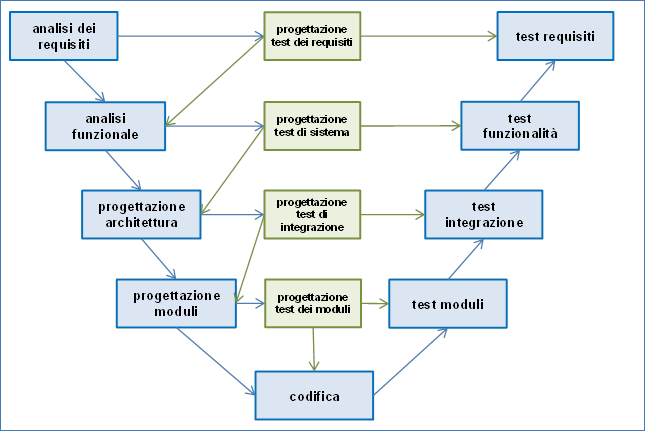
\includegraphics[width=12cm]{test_v.png}
\end{center}
\begin{center}
Immagine 1: Modello a V
\end{center}

\subsection{Tipologie di test}

\subsubsection{Test di unità}

I \textit{test di unità} sono un tipo di test che viene utilizzato per verificare il funzionamento di una singola unità di codice all'interno di un software.
Una unità di codice può essere una funzione, una classe o qualsiasi altra porzione di codice che
svolge una specifica attività all'interno del software.
Questa viene definita con l’inizio del processo di progettazione e sviluppo software.

\subsubsection{Test di integrazione}

I \textit{test di integrazione} sono un tipo di test che viene utilizzato per verificare il funzionamento delle diverse componenti di un software quando vengono integrate tra loro e sono particolarmente utili
per identificare e risolvere eventuali problemi di integrazione.
Inoltre, i \textit{test di integrazione} possono essere utilizzati per verificare che il software soddisfi i requisiti prestabiliti in modo completo e che sia pronto per essere messo in produzione.

\subsubsection{Test di sistema}

I \textit{test di sistema} vengono utilizzati per verificare il funzionamento del software come sistema
completo, inclusi tutti i componenti e le interfacce con gli altri sistemi. I test di sistema hanno lo
scopo di verificare che il software soddisfi i requisiti prestabiliti e che sia pronto per essere messo in
produzione. In particolare, questa tipologia di test mira a soddisfare tutti i requisiti funzionali e la maggior parte di quelli non funzionali, compresi aspetti relativi all’usabilità, sicurezza,
performance e vulnerabilità.

\subsubsection{Test di accettazione}

I \textit{test di accettazione} sono un tipo di test che viene utilizzato per verificare che il software soddisfi i requisiti prestabiliti dal capitolato e che sia pronto per essere consegnato al committente o messo in produzione.
Vengono svolti alla presenza del committente e mirano a soddisfare pienamente i requisiti,
accertandosi di avere un prodotto funzionante e soddisfacente le aspettative progettuali iniziali.

\subsubsection{Test di regressione}

I \textit{test di regressione} sono un tipo di test che viene utilizzato per verificare che le modifiche apportate ad un software non influiscano negativamente sulle sue funzionalità esistenti, sono particolarmente utili per garantire che il software continui a funzionare correttamente anche dopo aver apportato modifiche o aggiornamenti.
Consistono nella ripetizione selettiva di \textit{test di unità, integrazione e sistema}, verificando quindi di non perdere funzionalità nella progressiva realizzazione del prodotto software.


\subsection{Specifica dei test}
Al fine di garantire di creare una denominazione uniforme e per facilitare la comprensione, i test sono identificati da un codice come segue:
\begin{center}
    \textbf{T[Tipologia][Identificativo]}
\end{center}
Dove:
\begin{itemize}
    \item \textbf{Tipologia} indica il tipo del test eseguito:
    \begin{itemize}
        \item U: per Test di Unità;
        \item I: per Test di Integrazione;
        \item S: per Test di Sistema;
        \item A: per Test di Accettazione;
        \item R: per Test di Regressione.
    \end{itemize}
    \item \textbf{Identificativo} del test in oggetto
\end{itemize}
Ciascuna tipologia di test sarà rappresentata da apposite tabelle, comprensive di identificativo, descrizione e stato. Come riportato precedentemente, al momento sono stati effettuati esclusivamente i \textit{test di unità}.

\begin{comment}
    
    \subsubsection{Test di unità}

\begin{tblr}{
colspec={|X[2.5cm, halign=c]|X[9cm, halign=c]|X[3.5cm, halign=c]|},
row{odd}={bg=white},
row{even}={bg=white},
row{1}={bg=black, fg=white},
}
        Identificativo & Descrizione & Stato \\
        \hline
        TU1 & Si verifica che il componente DashboardClienti venga renderizzato correttamente & Superato \\
        \hline
        TU2 & Si verifica che il componente DashboardRistoratori venga renderizzato correttamente & Superato \\
        \hline
        TU3 & Si verifica che il componente DettagliPietanza venga renderizzato correttamente & Superato \\
        \hline
        TU4 & Si verifica che il componente DettagliPrenotazione venga renderizzato correttamente & Superato \\
        \hline
        TU5 & Si verifica che il componente FormPrenotazione venga renderizzato correttamente & Superato \\
        \hline
        TU6 & Si verifica che il componente MenuPietanze venga renderizzato correttamente & Superato \\
        \hline
        TU7 & Si verifica che il componente Navbar venga renderizzato correttamente & Superato \\
        \hline
        TU8 & Si verifica che il componente Login venga renderizzato correttamente & Superato \\
        \hline
        TU9 & Si verifica che il componente ListaOrdinazioni venga renderizzato correttamente & Superato \\
        \hline
        TU10 & Si verifica che il componente DashboardClienti visualizzi correttamente le prenotazioni del cliente & Superato \\
        \hline
        TU11 & Si verifica che il componente DashboardRistoratori visualizzi correttamente le prenotazioni del ristorante e permetta la loro gestione & Superato \\
        \hline
        TU12 & Si verifica che il componente DettagliPietanza visualizzi correttamente tutti i dettagli della pietanza e permetta l'ordinazione con l'eventuale rimozione di ingredienti & Superato \\
        \hline
        TU13 & Si verifica che il componente DettagliPrenotazione visualizzi correttamente i dettagli di ciascuna prenotazione e ne permetta la gestione & Superato \\
        \hline
        TU14 & Si verifica che il componente FormPrenotazione contsenta correttamente di effettuare una prenotazione & Superato \\
        \hline
        TU15 & Si verifica che il componente MenuPietanze visualizzi correttamente tutto il menù e permette l'ordinazione di ciascuna pietanza & Superato \\
        \hline
\end{tblr}

\begin{tblr}{
colspec={|X[2.5cm, halign=c]|X[9cm, halign=c]|X[3.5cm, halign=c]|},
row{odd}={bg=white},
row{even}={bg=white},
}
        \hline
        TU16 & Si verifica che il componente Navbar visualizzi correttamente la pagina attuale, le altre pagine e il nome dell'utente o del ristoratore loggato & Superato \\
        \hline
        TU17 & Si verifica che il componente Login permetta correttamente di effettuare l'accesso tramite cliente o ristoratore & Superato \\
        \hline
        TU18 & Si verifica che il componente ListaOrdinazioni visualizzi correttamente le ordinazioni confermate e l'inventario degli ingredienti & Superato \\
        \hline

\end{tblr}

\end{comment}


\section{Resoconto delle attività di verifica}

\subsection{Fornitura}

\subsubsection{MPC-AC e MPC-ETC: Actual Cost e Estimated to Completion}
\begin{figure}[H] 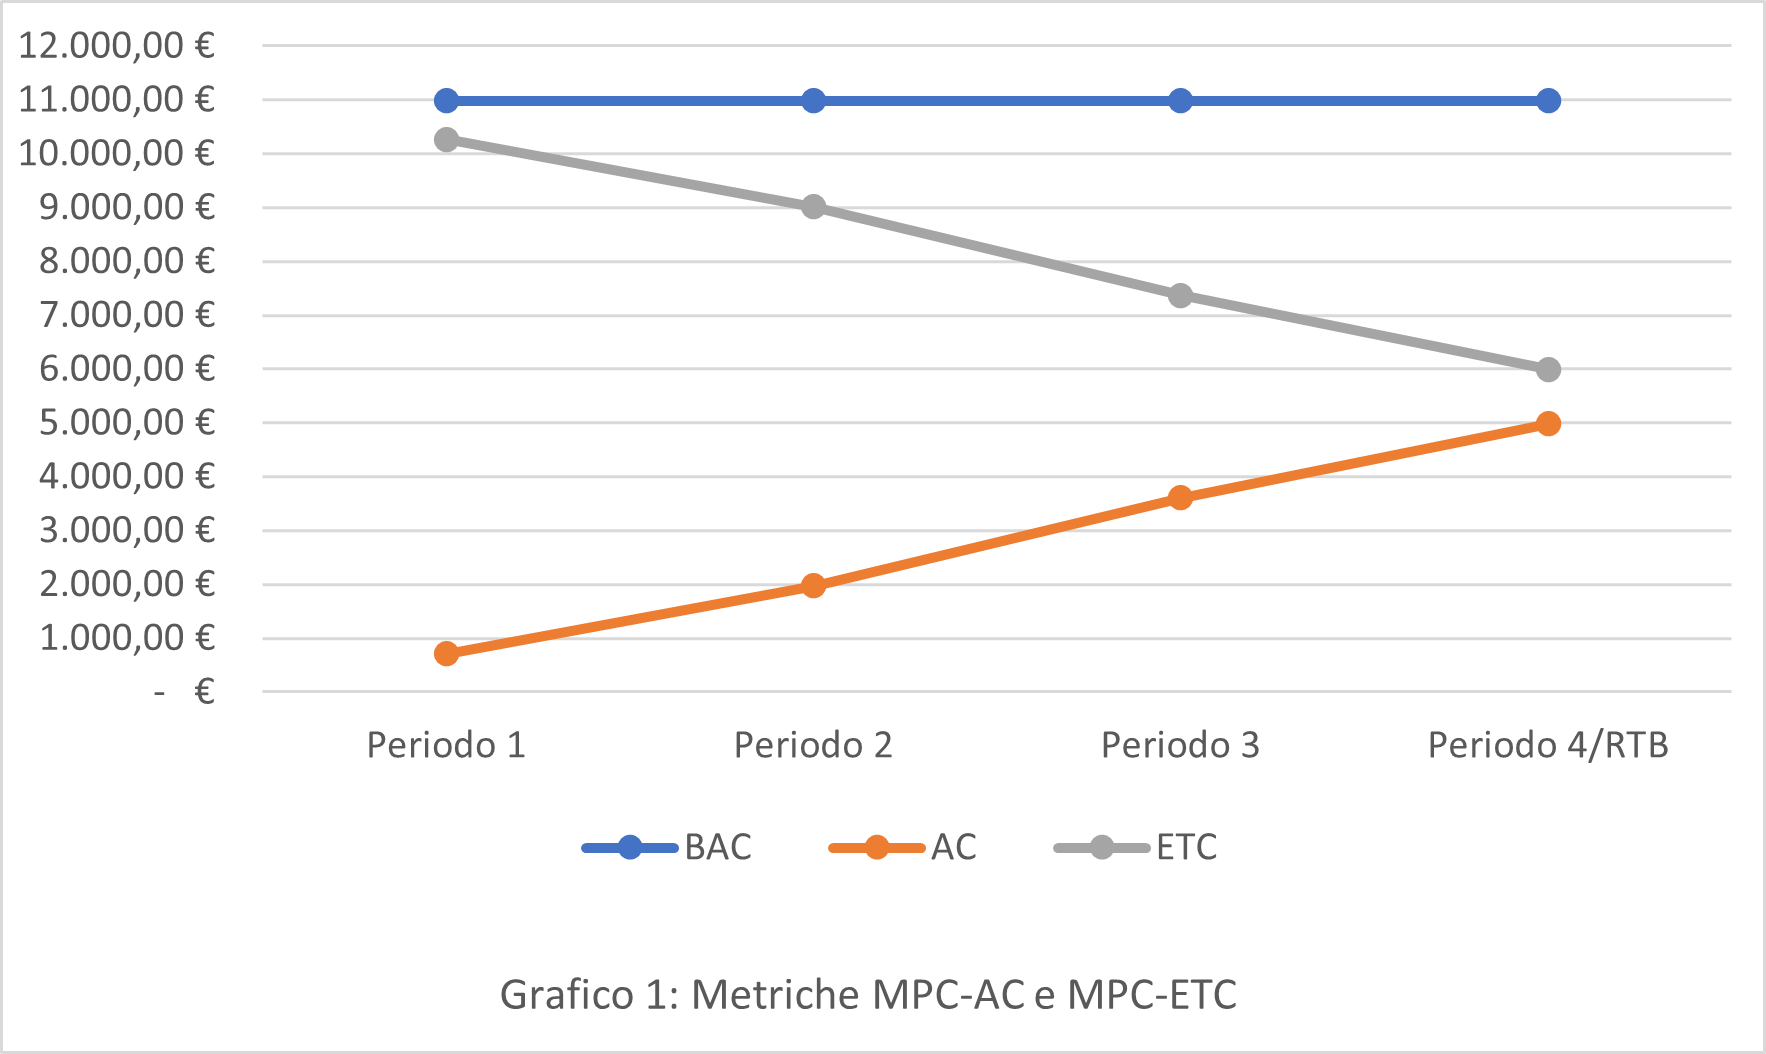
\includegraphics[scale=1]{i0.png} \end{figure}

\subsubsection{MPC-EV e MPC-PV: Earned Value e Planned Value}
\begin{figure}[H] 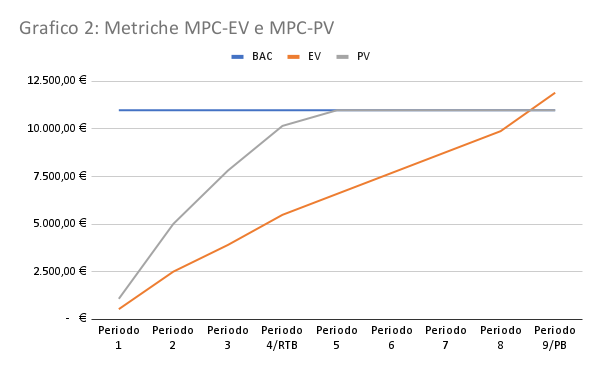
\includegraphics[scale=1]{i1.png} \end{figure}

\subsubsection{MPC-SV: Schedule Variance}
\begin{figure}[H] 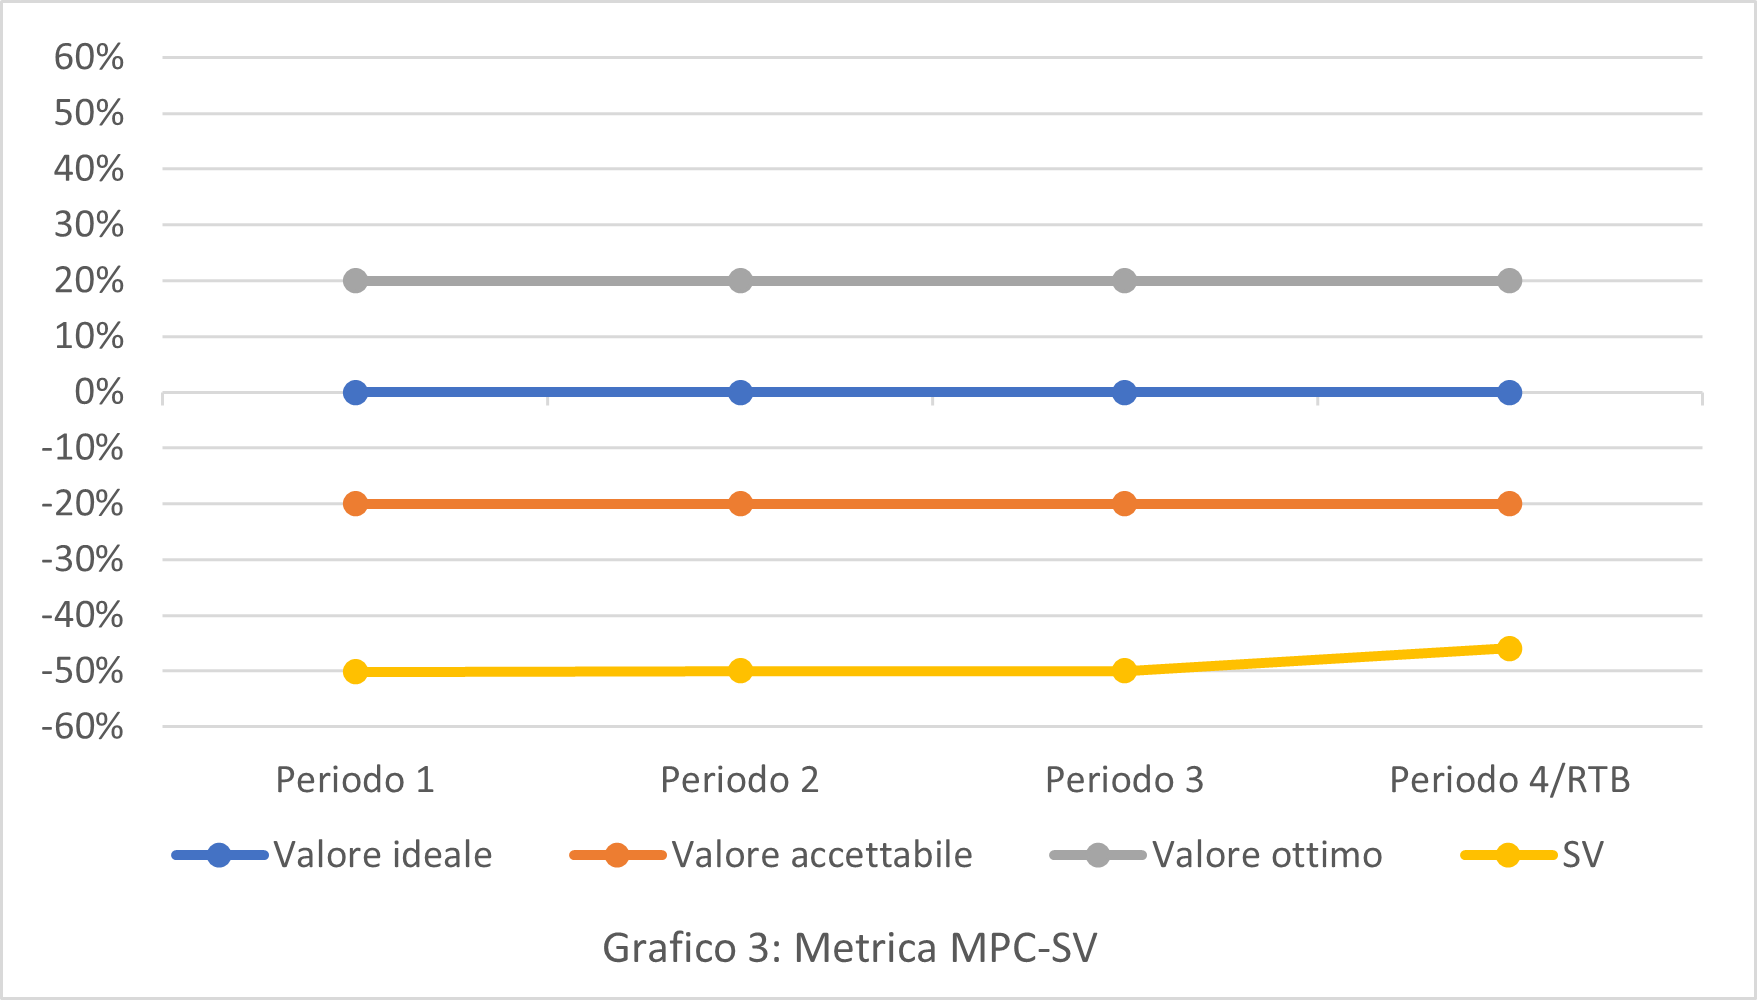
\includegraphics[scale=1]{i2.png} \end{figure}

\subsubsection{MPC-CV: Cost Variance}
\begin{figure}[H] 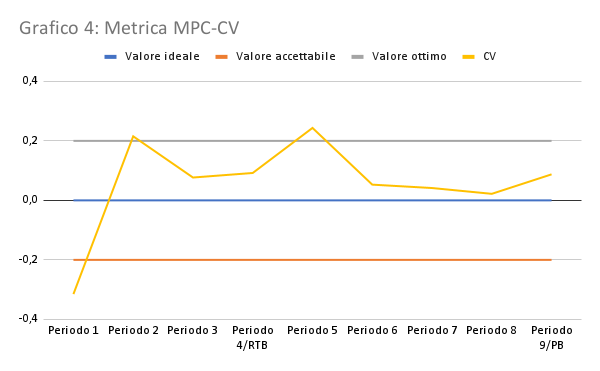
\includegraphics[scale=1]{i3.png} \end{figure}

\subsubsection{MPC-EAC: Estimated at Completion}
\begin{figure}[H] 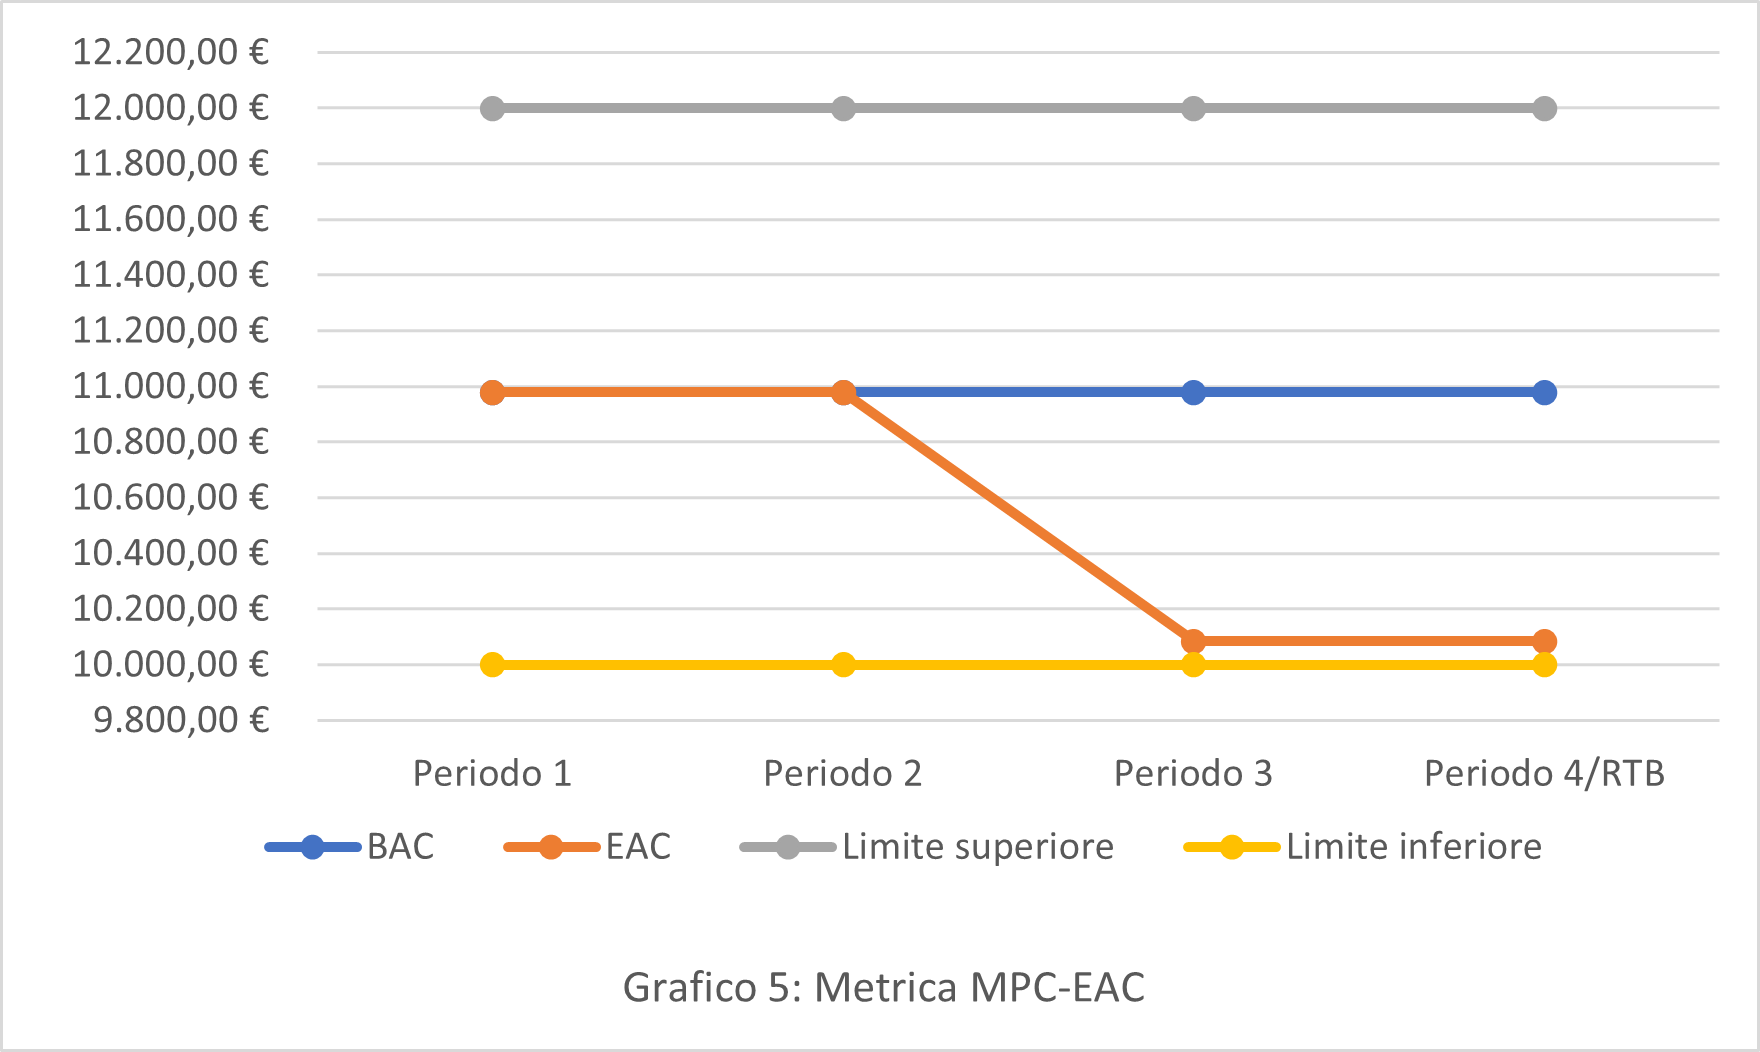
\includegraphics[scale=1]{i4.png} \end{figure}

\subsection{Documentazione}

\subsubsection{MPC-IG: Indice Gulpease}
\begin{figure}[H] 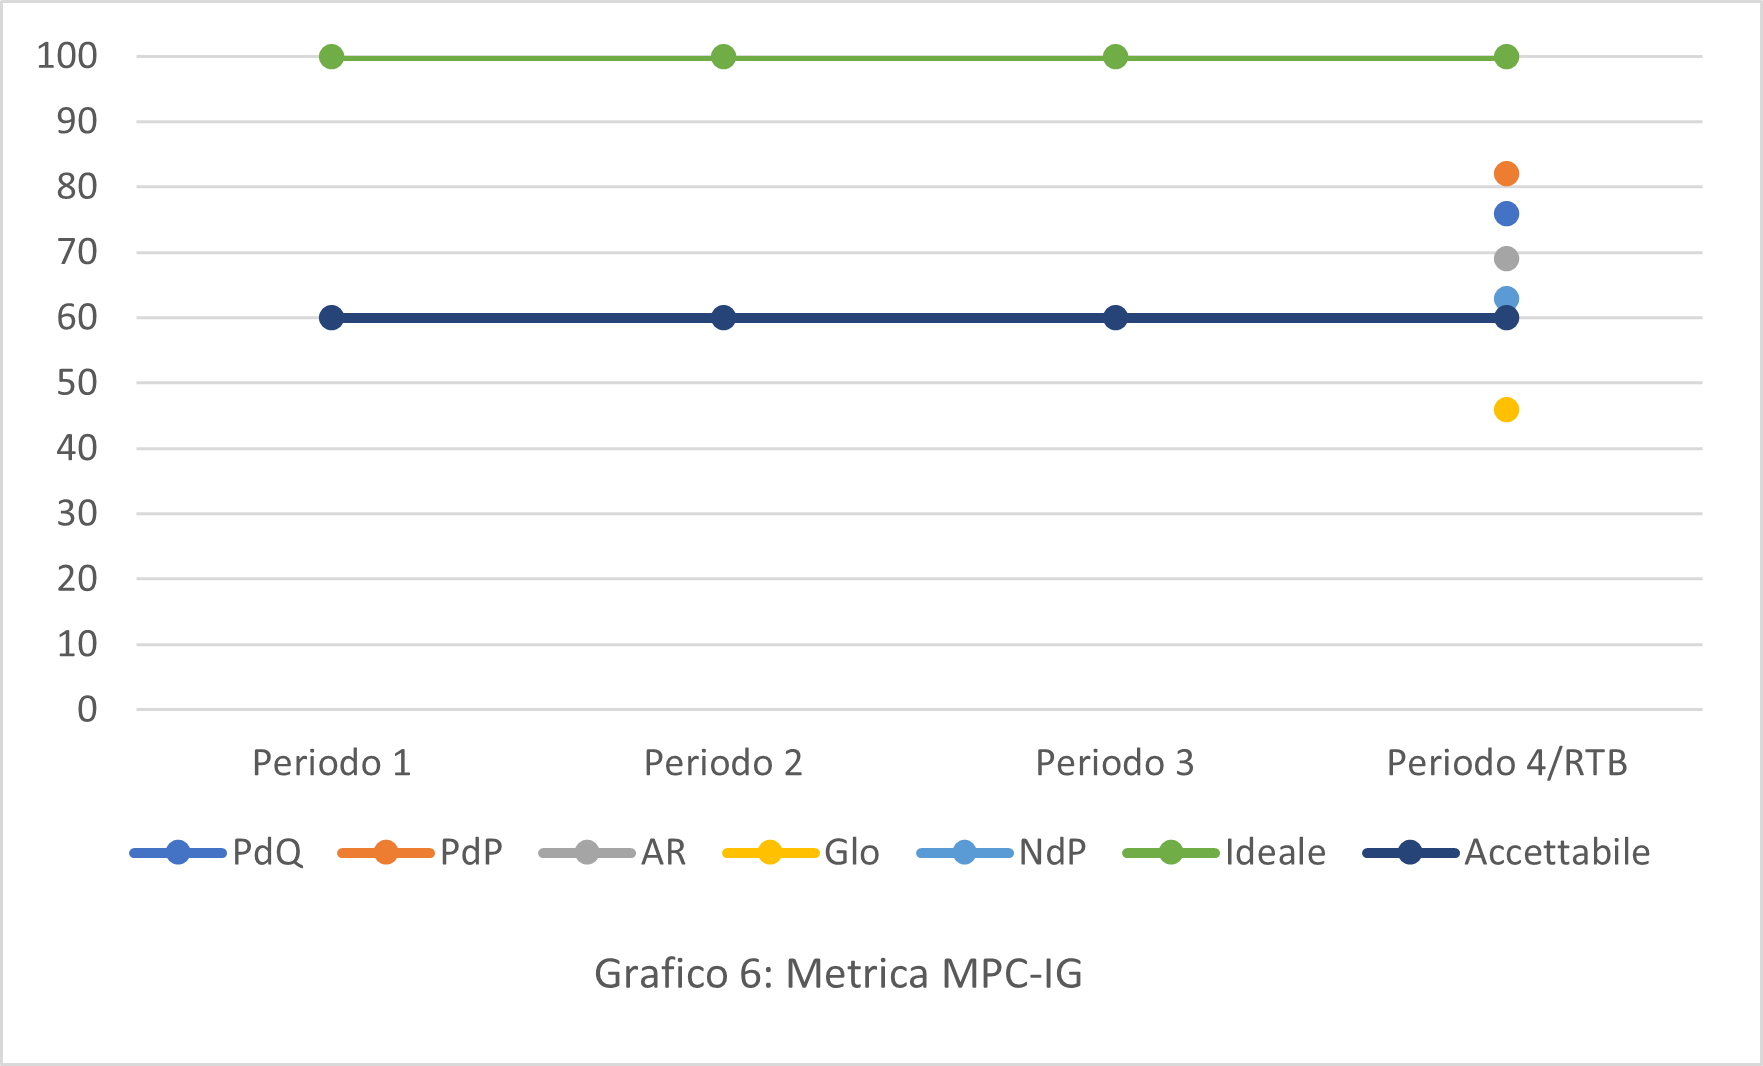
\includegraphics[scale=1]{d0.png} \end{figure}

%\subsubsection{MPC-CO: Correttezza Ortografica}
%\begin{figure}[H] 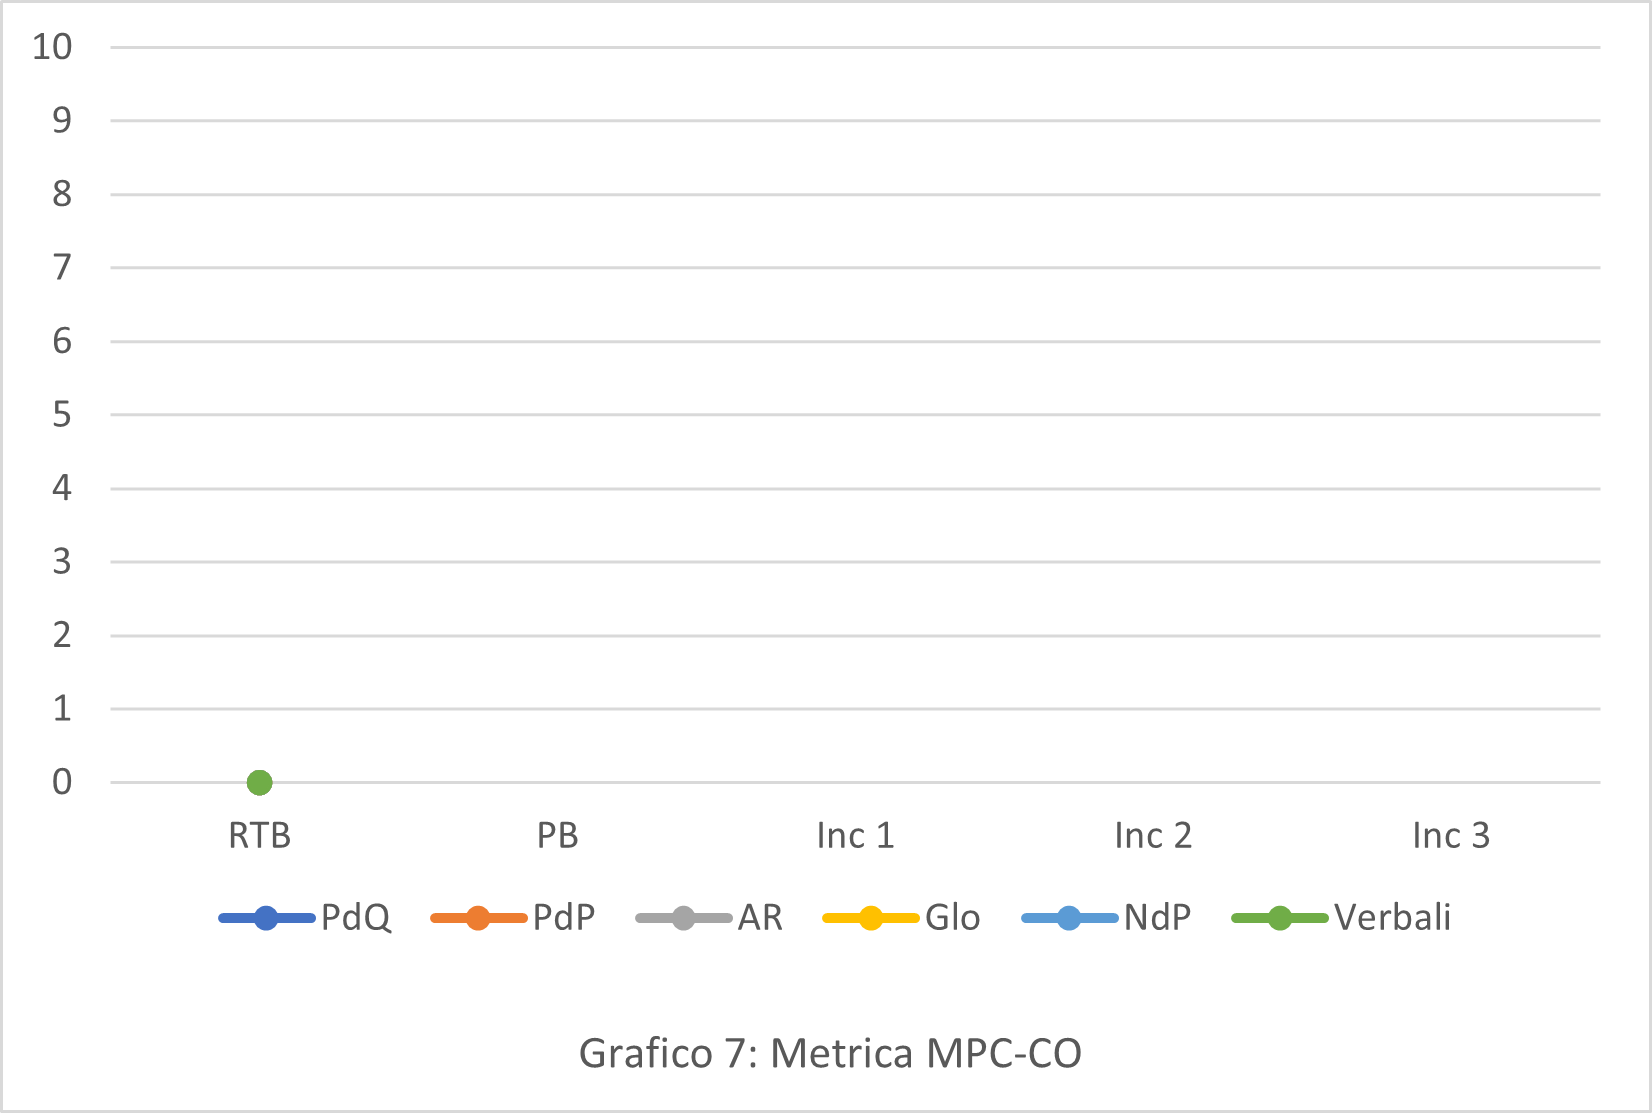
\includegraphics[scale=1]{d1.png} \end{figure}



\end{document}
